%O+I
% Dominic
% final

\ifx\wholebook\relax\else
\input{../Common.tex}
\input{../macroes.tex}
\begin{document}
\fi

\chapter{Composing Messages}\label{ch:Evaluating}\label{cha:evaluating}

As with any language,  \st follows certain rules to execute the messages sent to objects. We did not present them to you until now and you may have wondered how it works when you experimented the previous scripts. Your patience will be now rewarded. This chapter explains how to read and write correct messages. 

This chapter may look a bit more difficult or abstract than the previous ones. We did our best to present you the simple rules that govern how to write correct messages. We know that this may be not extremely fun but this is somehow the price to pay to be able to program more advanced. 
However to motivate you, first \st is not a complex language: there are only five rules to understand. You may also skip this chapter in a first reading and come back and read it when you will have questions about the way you write your programs. 


When you write a complex \emph{expression} such  as \ct{pica go: 100 + 20}, it contains \emph{several messages}: \ct{go:} and \ct{+} and you have to know the order in which these messages are executed.  In \st the order in which messages are executed is determined by the message kind. There are \emph{three} kinds of messages: \emph{unary}, \emph{binary}, and \emph{keyword-based} messages. Unary messages are always executed first, then binary messages and finally keyword-based ones. As parenthesized messages are executed prior to any other messages.  We can then change the execution order of message sequence using parenthesis. These rules make reading \st code as easy as possible. And most of the time you do not have to think about them. However, you have to know them because there are occasions where you will have to use them.  

Note that we payed attention that all the examples we show you can be executed as shown in the text. Therefore do not hesitate to execute the examples. We start by showing you how to identify the different kinds of messages, then we give some examples of each kind and finally we show how message composition rules. 

\section{Identifying Messages}

When you write a complex \emph{expression} such  as \ct{pica go: 100 + 20}, it contains \emph{several messages}: \ct{go:} and \ct{+}. As described in Chapter~\ref{cha:firstscript},  a message is a pair composed of the selector message and the optional message arguments. \st defines a couple of simple rules to determine the order in which the messages are executed. These rules, which we shall present in detail after, are based on the distinction between 3 different kinds of messages: 

\begin{itemize}
\item \index{unary messages}\textit{unary messages} are messsages sent to an object without any other information. For example in \ct{\caro color}, \ct{color} is a unary message. The message \ct{color} does not require any other information.

\item  \index{binary messages}\textit{binary messages} \ie messages mainly related to mathematical expressions. Note that binary means two thus binary messages are messages that imply two objects: the message receiver and another object. For example in \ct{10 + 20}, \ct{+} is a binary message sent to the object \ct{10} with the object \ct{20}. 

\item  \index{keyword-based messages} \textit{keyword-based messages} \ie messages that contain at least one colon character \ct{:} in their names and involved more than one object. For example in \ct{pica go: 100}, \ct{go:} contains the character \ct{:} and two objects, \caro and \ct{100}, are involved in the message. 
 \end{itemize}
 
The first step is to identify messages and their receiver. To help you we propose you to use a graphical notation as shown in Figure~\ref{fig:ellipse}. In all the figures of this chapter, we underline the message receivers. We also surround each message in an ellipse and number the expression starting from the first expression that will be executed. When there are several ellipses we dashed them. This way you can see how messages are executed.

Figure~\ref{fig:ellipse} represents one expression composed of two expressions \ct{Color yellow} and \ct{\caro color: Color yellow} hence there are two ellipses one plain and one dashed. The expression \ct{Color yellow} is executed first so its ellipse is numbered as \ct{1}.  There are two receivers: \ct{\caro} which receives the message \ct{color: ...} and \ct{Color} which receives the message \ct{yellow} therefore they are both underlined.

\begin{figure}[!h]
\centerline{\includegraphics[width=8cm]{ukeyUnOne}} 
\caption{\ct{\caro color: Color yellow} is composed of two expressions: \ct{Color yellow} and \ct{\caro color: Color yellow}. The message \ct{yellow} is sent to \ct{Color} and the message \ct{color: ...} is sent to \ct{\caro}\label{fig:ellipse}}
\end{figure}


Every message is sent to an object that is called the  \index{message receiver} \index{receiver} \textit{message receiver}. Note that receivers are not limited to be graphical robots but can be anything from numbers to windows. 
A message receiver can be the first element of a message as \ct{\caro} in the expression \ct{\caro go: 100} or \ct{Color} in the expression \ct{Color new}. However, a receiver can also be the result of other messages. For example in the message \ct{\Turtle new go: 100}, the receiver of the message \ct{go: 100} is the resulting object returned by the expression \ct{\Turtle new}. In all the cases, a message is always sent to an object named the \emph{message receiver} which may be the result of another message. 

\begin{largecadre}{A message is always sent to an object named the \emph{message receiver} which may be the result of other messages.}\end{largecadre}

  
 \Tscrref{scr:messageExamples} shows some messages and we suggest you to try identify to which kind they belong to and to draw the graphical representation of the message. 
 
\begin{scriptwithtitle}{Examples of Messages}\label{scr:messageExamples}
\begin{tabbing}
aaaaaaaaaaaaaaaaaaaaaaaaaaaaaaaaaaaaaaaaaaaannnnnnaaaaaaaa\=aaaaaaaaaaaaaaaaaaaaaa\kill
\caro go: 100.							\> keyword-based\\
"the receiving robot moves forward 100 pixels"\\
\\
100 + 20      						\>binary\\
"the number 100 receives the message + with the number 20"\\
\\
\caro east\>unary\\
"the receiving robot points to the east"\\
\\
\caro color: Color yellow\>keyword-based and unary\\
"the receiving robot changes its color to the color yellow"\\
\\
\caro go: 100 + 20\>keyword-based and binary\\
"the receiving robot moves forward 120 pixels"\\
\\
\Turtle new go: 100\> unary and keyword-based\\
"The message new is sent to the \Turtle class which 
returns a new robot to which is sent go: 100"
\end{tabbing}
\end{scriptwithtitle}


From the script~\ref{scr:messageExamples} you should see that: 
\begin{enumerate}
\item There are messages with arguments or not. \ct{east} does not have argument, \ct{go: 100} and \ct{+ 20} have one argument the number \ct{20}. 
\item There are messages sent to different objects. In  \ct{\caro east} the message is sent to a robot and in \ct{100 + 20} the message is sent to the number \ct{100}.
\item There are simple messages and composed ones. \ct{Color yellow} and \ct{100 + 20} are  simple:  a message is sent to an object, while the expression \ct{\caro go: 100 + 20} is composed of two messages: \ct{+ 20} is sent to \ct{100} and \ct{go: 100 + 20} sent to \caro and using the result of the execution of the first message.
\item A message receiver can be an expression which returns itself an object. In \ct{\Turtle new go: 100}, the message \ct{go: 100} is sent to the object that results from the evaluation of the expression \ct{\Turtle new}.
\end{enumerate}


\section{Three Kinds of Messages}
Now that you can identify message receivers and the kind of message let us look at them in detail. 


\subsection*{Unary Messages} 
Unary messages are messages that do not require any argument beside the message receiver. They are often used to get some results.  They are of the form of \ct{receiver methodName}. \Tscrref{scr:unary} presents some examples of unary messages. 

\begin{scriptwithtitle}{Examples of Unary Messages}\label{scr:unary}
| \caro |
\caro := \Turtle \textbf{new}.
\caro \textbf{color}.
\caro \textbf{penSize}.
\caro \textbf{east}.
Color \textbf{yellow}
125 \textbf{factorial}
\end{scriptwithtitle}

\begin{largecadre}{Unary messages are messages that do not require any argument.\\
They are of the form of \ct{receiver methodName}}
\end{largecadre}

\subsection*{Binary Messages} The term binary means two. Binary messages are messages that involve two objects, the receiver and another object \textit{and} whose method name are composed of  one or two characters from the following list: \ct{+}, \ct{-}, \ct{*}, \ct{/}, \ct{|}, \texttt{\&}, \ct{=}, \ct{>}, \ct{<}, \texttt{\~}, and \ct{@}.
Therefore \ct{+}, \ct{=} or \ct{*} are messages but also \ct{=>} which is composed of two symbols.


\Tscrref{scr:binary} shows some examples of binary messages and their meaning. Note that we do not want to go into the details of the examples given, so do not worry if you do not understand precisely all the examples but try them out.



\begin{scriptwithtitle}{Examples of Binary Messages on Numbers}\label{scr:binary}
\begin{tabbing}
aaaaaaaaaaaaaaaaaaaaaaaaaaaaaaaaaaaaaaaaaaaaa\=aaaaaaaaaaaaaaaaaaa\kill
1 \textbf{+} 2.5           \>"Addition of two numbers"\\
\pr 3.5                   \\
3.4 \textbf{*} 5                               \>"Multiplication of two numbers"\\
\pr 17.0\\
8 \textbf{/} 2                               \>"Division of two numbers"\\
\pr 4\\
10 \textbf{-} 8.3                       \>"Substraction of two numbers"\\
\pr 1.7\\
12 \textbf{=} 11                     \>"Equality between two numbers"\\
\pr false\\
12 \textbf{~=} 11                \>"Testing is two number are different"\\
\pr true\\
12 \textbf{>} 9                 \>"Greater than"\\
\pr true\\
12 \textbf{>=} 10          \>"Greater or equal  than"          \\
\pr true\\
12 \textbf{<} 10         \>"Smaller  than"\\
\pr false\\
100\textbf{@}10     \>"Point creation"\\
\pr 100@10
\end{tabbing}
\end{scriptwithtitle}

\begin{largecadre}{Binary messages are messages that involve two objects, the receiver and another object \textit{and} whose method name are composed of  one or two characters from the following list: \ct{+}, \ct{-}, \ct{*}, \ct{/}, \ct{|}, \texttt{\&}, \ct{=}, \ct{>}, \ct{<}, \texttt{\~}, and \ct{@}.
They are of the form: \ct{receiver methodName argument}}
\end{largecadre}

\subsection*{Keyword-based Messages} 
Keyword-based messages are messages that involve more than one objects and that contain at least one character~\ct{:}. Note that the name of the method includes the~\ct{:}, hence the method name is \ct{go:} and not \ct{go}. 

\begin{scriptwithtitle}{Examples of Keyword-based Messages.}\label{scr:keyword}
| \caro |
\caro := \Turtle new.
\caro \textbf{go:} 100.
\caro \textbf{penSize:} 5.
\caro \textbf{color:} Color yellow.
\caro \textbf{turn:} 90
\end{scriptwithtitle}

Keyword-based messages can have multiple arguments. For example, the method \ct{aNumber between: lowerBound and: upperBound} that checks whether a number is in the interval represented by two numbers needs two arguments, the two bounds of the interval as shown in \tscrref{scr:keyword2}. Note the method name is \ct{between:and:} and is composed of the two words \ct{between:} and \ct{and:}. 

\begin{scriptwithtitle}{An example of keyword-based messages with multiple arguments}\label{scr:keyword2}
5 \textbf{between:} 2 \textbf{and:} 10
\pr true
Color \textbf{r:} 0 \textbf{g:} 1 \textbf{b:} 0
\end{scriptwithtitle}

\begin{largecadre}
{Keyword-based messages are messages that involve more than one objects and that contain at least one character~\ct{:}. They are of the form: \ct{receiver \textbf{methodNameWordOne:} argumentOne\\   
       \textit{\textbf{wordTwo:} argumentTwo}}}
\end{largecadre}

\section{Composing Messages}\label{sec:composing}

We saw that there are  three kinds of messages: unary, binary, and keyword-based. 
The message execution order is determined by the type of the message as  described by the three following rules:

\begin{itemize}
\item[(1)] Unary messages are always executed first, then binary messages and finally keyword-based ones. 
\item[(2)] Similar to  mathematical expressions, messages in parentheses are executed prior to any kind of messages. 
\item[(3)] Messages of the same kind messages are evaluated from left to right. 
\end{itemize}

You can think that these rules are complex but they are natural and you do not have to think too much of them most of the time. In particular, the third rule example follows the reading order. 

If you want to be sure that your messages are executed the way you want you can always put more parenthesizes as shown by the Figure~\ref{fig:ukeyUn}. In this  figure, the message \ct{yellow} is an unary message and the message \ct{color:} a keyword-based one, therefore the expression \ct{Color yellow} is executed first. However as expressions in parenthesis are executed first putting parentheses around \ct{Color yellow} makes sure that it will be executed first. The rest of the section illustrates each of  these points.




\begin{figure}[h]
\centerline{\includegraphics[width=10cm]{ukeyUn}} 
\caption{Unary messages are executed first so \ct{Color yellow} is executed, this execution returns a color object which is passed as argument of the message \ct{\caro color:}.\label{fig:ukeyUn}}
\end{figure}



\section*{Unary > Binary > Keywords}
Unary messages are executed first then binary messages, and finally keyword-based messages. In programmer jargon we also say that unary messages have a higher  priority over the other kind of messages.


\begin{largecadre}
{\textbf{Rule One.} Unary messages are executed first, then binary messages, and finally keyword-based messages.}
\end{largecadre}

\paragraph{Example 1.}
In the message \ct{\caro color: Color yellow}, there is one \emph{unary} message \ct{yellow} sent to the class \ct{Color} and a \emph{keyword-based} message \ct{color:} sent to \ct{\caro}.  Unary messages are executed first so the expression \ct{Color yellow} is executed (1), this execution returns a color object which is passed as argument of the message \ct{\caro color: aColor} (2). Figure \ref{fig:ukeyUn} shows graphically how messages are executed.

\newpage
Now to help you, we propose another textual way to represent the step by step expression execution. \exeref{scr:decColor} is such a textual representation that we explained just after. 

\begin{decomp}{Decomposing the execution of \ct{\caro color: Color yellow}}\label{scr:decColor}
\begin{tabbing}
aaaaaaaaaaaaaaaaaaaaaaaaaaaaaaaaaaaaaaaaa\=aaaaaaaaaaaaaaaaaa\kill
     \textbf{\caro color: Color yellow}\\\\
(1)                    Color yellow\>"unary"\\
                     \returns \emph{aColor}\\
(2)  \caro color: \emph{aColor}\>"keyword-based"
\end{tabbing}
\end{decomp}

The first line contains the complete expression in bold that we want to execute step by step. In \exeref{scr:decColor} we want to execute step by step the expression \ct{\caro color: Color yellow}. 

The following lines represent the execution steps in the order they will occur: an expression on the top is executed before one expression down. The numbers in parenthesis at the beginning of a line indicate the step in which the expressions are executed. For example \ct{Color yellow} is the first expression to be executed. Note that the horizontal placement follows the placement of the main expression. 

When an expression execution returns a result that is used in the following execution, the line following the executed expression contains a \returns with the result. Here the expression \ct{Color yellow} returns an object color that we name \ct{aColor}. 
The second expression to be executed is \ct{pica color: aColor}, here \ct{aColor} is the result obtained from the previous execution step. To stress this point the returned value or object are displayed in italic. To help you, we put between comments \ct{"} the kind of message that is currently executed. For example \ct{Color yellow} is a unary message.

 





%\begin{figure}
%\centerline{\includegraphics[width=8cm]{ukeyBin}} 
%\caption{Binary messages are executed prior to keyword-based messages so \ct{100 + 20} is executed, the message \ct{+ 20} is sent to the object \ct{100} which results in the number \ct{120}. Then the message \ct{\caro go:} is executed with \ct{120} as argument.\label{fig:keyBin}}
%\end{figure}


\paragraph{Example 2.} In the message \ct{\caro go: 100 + 20}, there are a \emph{binary} message \ct{+ 20} and a \emph{keyword-based} message \ct{go:}. Binary messages are executed prior to keyword-based messages so \ct{100 + 20} is executed (1), the message \ct{+ 20} is sent to the object \ct{100} and returns the number \ct{120}. Then the message \ct{\caro go: 120} is executed with \ct{120} as argument (2).
\Tscrref{scr:decGo} shows the way the expression is executed. 

\

\begin{decompfigwithsize}[0.65]{\includegraphics[width=6cm]{ukeyBin}}{Decomposing \ct{\caro go: 100 + 20}}\label{scr:decGo}
      \textbf{\caro go: 100 + 20}
      
(1)                  100 + 20                        "binary"
                   \returns  120
(2)  \caro go: 120                                 "keyword-based"
\end{decompfigwithsize}




\paragraph{Example 3.}
The message \ct{\caro penSize: \caro penSize + 2} contains one unary message \ct{penSize}, one binary message \ct{+},  and one keyword-based message \ct{penSize:}.
The unary message \ct{\caro penSize} is executed first (1), this message returns a number representing the current size of the receiver pen. Then the binary message is executed (2), the returned number is sent the message \ct{+ 2} which in its turn returns another number. Finally the keyword-based message 
\ct{penSize:} is executed with the last number as argument. The expression increases the receiver pen size by two pixels. \Tscrref{scr:decpen} illustrates the decomposition of message execution.


\

\begin{decompfigwithsize}[0.65]{\includegraphics[width=6cm]{ukeyUnBin}}{Decomposing \ct{ \caro penSize: \caro penSize + 2}}\label{scr:decpen}
   
      \textbf{\caro penSize: \caro penSize + 2}
(1)                          \caro penSize                    "unary"
                          \returns aNumber
(2)                           aNumber + 2	                  "binary"
                           \returns  anotherNumber	
(3)   \caro penSize: anotherNumber                 "keyword"      
\end{decompfigwithsize}




\paragraph{Example 4.} As an exercise we let you decompose the execution of the message \ct{\Turtle new go: 100 + 20} which is composed of one unary, one keyword-based and one binary message (see Figure~\ref{fig:unKeyBin}).
% The unary message \ct{\Turtle new} is first executed. It returns a new bot, then the binary message \ct{100 + 20} is executed and returns \ct{120}. Finally the message \ct{go:} is sent to the newly created robot with \ct{120}.

\begin{figure}[h]
\begin{center}
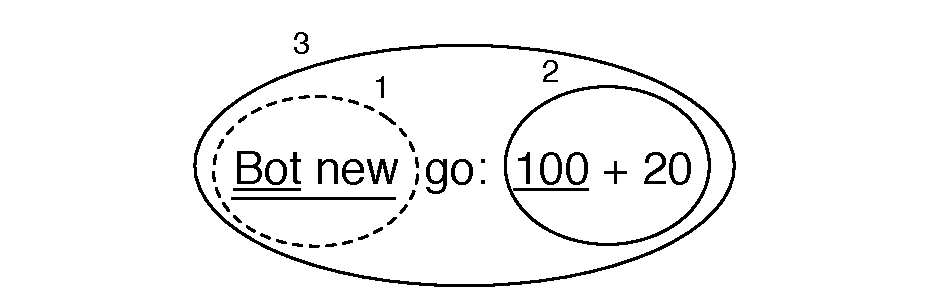
\includegraphics[width=6cm]{uunKeyBin}
\caption{Decomposing \ct{\Turtle new go: 100 + 20}}\label{fig:unKeyBin}
\end{center}
\end{figure}

\section*{Parentheses First}
The default ordering of message execution may not fit what we want, therefore we should be able to change it. For this purpose, \st offers parentheses \ct{(} and \ct{)}. Similar to mathematics, expressions in parentheses are executed before the others. 

Note that if you find the rules we explained a bit complex, use parenthesis to make sure that the messages are executed the way you want. Figures~\ref{fig:uKeyUnBinPar} shows some of the previous expressions and their equivalent using parenthesises. 

\begin{largecadre}{\textbf{Rule Two.} Similar to mathematics, expressions in parentheses are executed before the others. }
\end{largecadre}

\paragraph{Example 5.}
The message \ct{(65@325 extent: 134 @ 100) center} returns the center of a rectangle whose left top point is 65,325 and whose size is 134 and 100. \exeref{scr:decExtent} shows how the message is decomposed and sent. First the message between parentheses is executed: it contains two binary messages \ct{65@325} and \ct{134@100} that are executed first and return points, and a keyword-based message \ct{extent:} which is then executed and returns a rectangle. Finally the unary message \ct{center} is sent to the rectangle and a point is returned. 
Evaluating the message without parenthesis leads to an error because the object \ct{100} does not understand the message \ct{center}.

\begin{decomp}{Decomposing with Parentheses Priority.}\label{scr:decExtent}
      \textbf{(65 @ 325 extent: 134 @ 100) center}
      
(1)   65@325                                                                    "binary"
   \returns \emph{aPoint}
(2)                                134@100                                     "binary"
                                 \returns \emph{anotherPoint}
(3)   \emph{aPoint} extent: \emph{anotherPoint}                                       "keyword-based"
   \returns \emph{aRectangle}
(4)   \emph{aRectangle} center                                                     "unary"
   \returns 132@375
\end{decomp}

%To prove yourself that you understand the way message execution works, try to execute this message 
%as if it would not have parenthesis. You should be able to find why the following expression that compare two points \ct{100@200 = 200@300} should be written \ct{100@200 = (200@300)}.



\section*{From Left to Right}
Now we know how messages from different kinds or priorities are handled. The final question to be addressed is how messages with the same priority are executed. They are executed from the left to the right. Note that you already saw this behavior in the script~\ref{scr:decExtent} where the two points creation (\ct{@}) were
executed first.



\begin{largecadre}{\textbf{Rule Three.} When the messages are of the same kind, the order of execution is from left to right.}
\end{largecadre}

%\begin{figure}
%\centerline{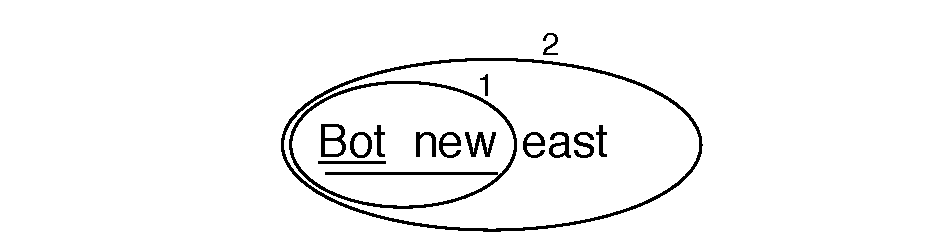
\includegraphics[width=8cm]{ucompoUn}} 
%\caption{The message \ct{\Turtle new east} is composed of two unary messages. Therefore the leftmost one, \ct{new},  is executed and it returns a new robot to which the second message \ct{east} is sent. \label{fig:compoUn}}
%\end{figure}

\paragraph{Example 6.} In the expression \ct{\Turtle new east} all messages are unary messages, so the first one \ct{\Turtle new} is executed first, it returns a newly created robot to which the second message \ct{east} is sent. \exeref{scr:unaryMessages} shows this execution.

%\begin{scriptwithtitle}{Evaluating unary messages}\label{scr:unaryMessages}
%     \Turtle new east 
%  (1)  \Turtle new          "unary"
%       \returns aBot
%  (2)  aBot east        "unary"
%\end{scriptwithtitle}


%The message \ct{\Turtle new east} is composed of two unary messages. Therefore the leftmost one, \ct{new},  is executed and it returns a new robot to which the second message \ct{east} is sent.
\

\begin{decompfigwithsize}[0.5]{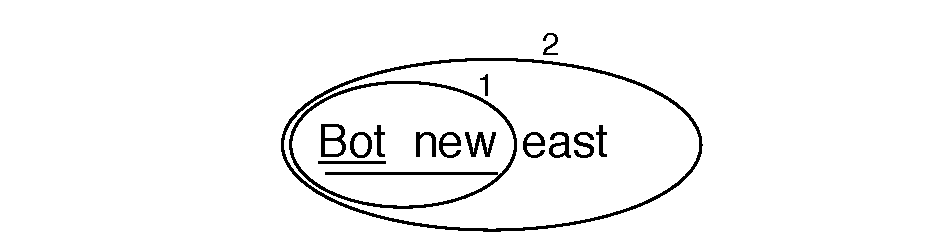
\includegraphics[width=8cm]{ucompoUn}}{Decomposing \ct{\Turtle new east}}\label{scr:unaryMessages}
        \textbf{\Turtle new east}
        
  (1)  \Turtle new                 "unary"
      \returns  \emph{aBot}
  (2)         \emph{aBot} east        "unary"
\end{decompfigwithsize}




\paragraph{Example 7.} 
In the expression \ct{20 + 2 * 5}, there are only binary messages \ct{+} and \ct{*}. However in \st there is no specific priority for mathematical operation, \ct{+} and \ct{*} are just binary messages. Therefore,  \ct{*} does not have priority over \ct{+}. Here the leftmost message \ct{+} is sent first (1) and then the \ct{*} is sent to the result as shown in \exeref{scr:binaryMessages1}.  


\  

\begin{decompfigwithsize}[0.6]{
\includegraphics[width=8cm]{ucompoNoBracketPar}}{Decomposing \ct{20 + 2 * 5}}\label{scr:binaryMessages1}
As there is no priority among binary messages, the leftmost message \ct{+} is evaluated first even if mathematically the \ct{*} should have be executed first. 

      \textbf{20 + 2 * 5}
  
(1)  20 + 2
  \returns 22
(2)  22 * 5
   \returns 110
\end{decompfigwithsize}

Hence as shown in \exeref{scr:binaryMessages1} the result of this expression is not \ct{30} but \ct{110}. This behavior is really unexpected but derives simply from the rules used to execute messages. This is somehow the price to pay for the simplicity of the \st model which has only methods. To get the mathematically correct result, we should use parenthesis. When messages are enclosed they evaluated first. Hence the expression \ct{20 + (2 * 5)} returns the mathematical result as shown in \exeref{scr:mathcorrect}. 

\


\begin{decompfigwithsize}[0.6]{
\includegraphics[width=8cm]{ucompoNumberBracket}}{Decomposing \ct{20 + (2 * 5)}}\label{scr:mathcorrect}
The messages surrounded by parenthesis are evaluated first therefore \ct{*} is executed prior than \ct{+} which produces the correct mathematical behavior.

         \textbf{20 + (2 * 5)}
(1)              2 * 5
               \returns 10
(2)    20 + 10
     \returns 30
\end{decompfigwithsize}


\largecadre{In \st, traditional mathematical operators such as + and * do not have different priority. \ct{+} and \ct{*} are just binary messages, therefore \ct{*} does not have priority over \ct{+}. We should use parenthesis to obtain the correct result.}

\begin{astuce}
The fact that \st does not follow mathematical precedence can be confusing at the beginning. Therefore, when you have multiple binary messages representing mathematical expression, just put parenthesis to express how the computation should be performed. When you will be accustomed to the way the messages are executed, you will simply start to be lazier and just put the exact number of parenthesis. 
\end{astuce}

\begin{figure}
\begin{center}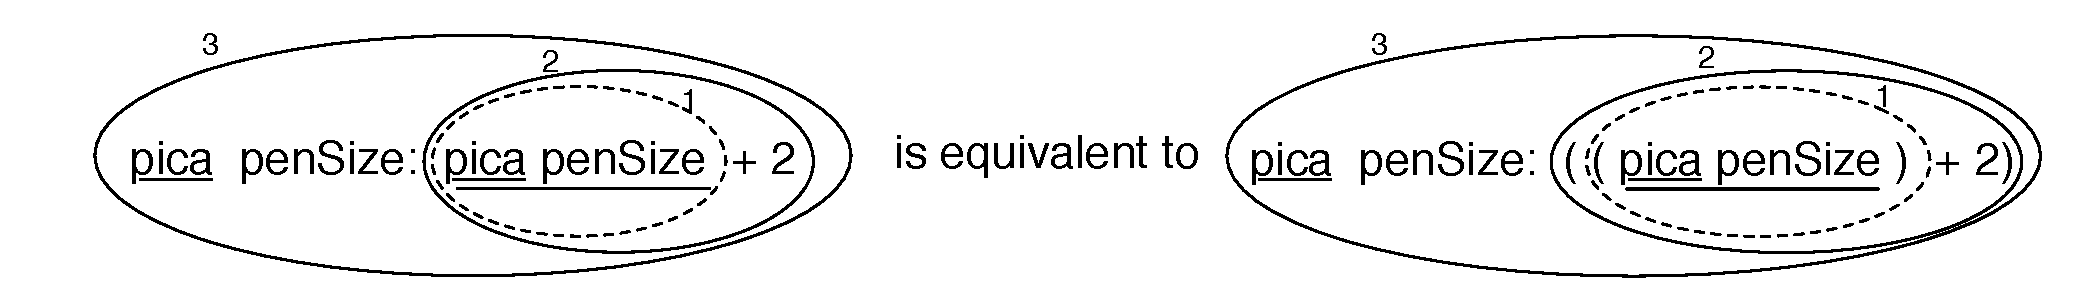
\includegraphics[width=10cm]{uKeyUnBinPar}
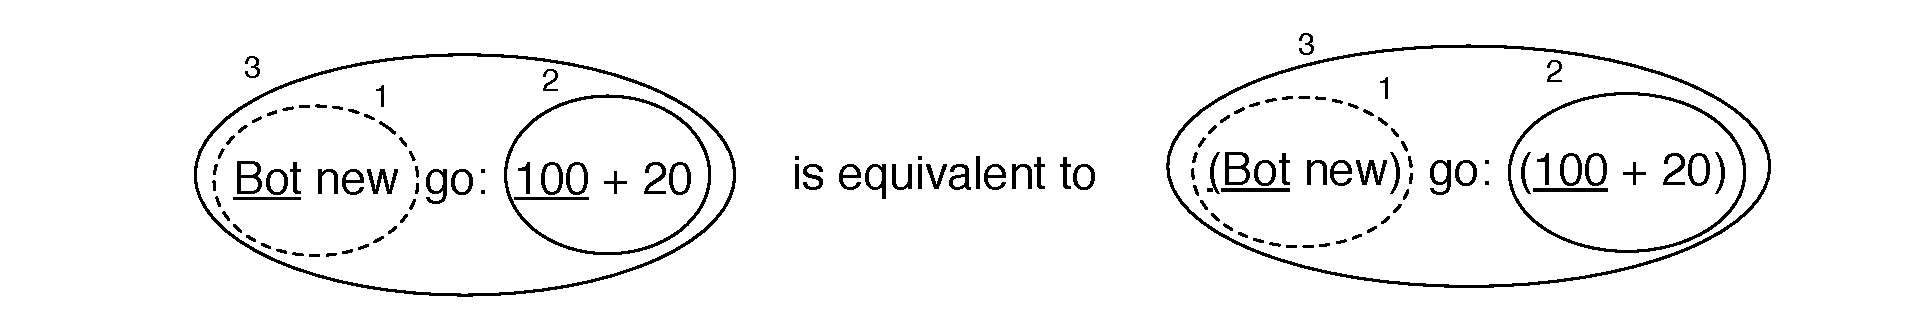
\includegraphics[width=10cm]{uunKeyBinPar}\end{center}
\caption{Equivalent messages using parenthesis. \label{fig:uKeyUnBinPar}}
\end{figure}


Note that the first rule stating that unary messages are executed prior to binary and keyword-based messages avoids to have to put explicit parentheses around. Therefore most of the time, you do not have to worry. \scrref{scr:expressions} shows expressions written following the rules and equivalent expressions if the rules would not exist, both expressions are resulting in the same effect or returning  the same value. 

\begin{scriptwithtitle}{Expressions and their equivalence fully parenthesized}\label{scr:expressions}
\begin{tabbing}
aaaaaaaaaaaaaaaaaaaaaaaaaaaaa\=aaaaaaaaaaaammmmmmm\=aaaaaaa\kill
\caro color: Color yellow\>is equivalent to\>\caro color: (Color yellow)\\
\caro go: 100 + 20\>is equivalent to\>\caro go: (100 + 20) \\
\caro penSize: \caro penSize + 2\>is equivalent to\>\caro penSize: ((\caro penSize) + 2)\\
2 factorial + 4\>is equivalent to\>(2 factorial) + 4
\end{tabbing}
\end{scriptwithtitle}


\summa

\begin{itemize}
\item A message is always sent to an object named the message receiver which may be the result of other messages.

\item Unary messages are messages that do not require any argument.\\
They are of the form of \ct{receiver methodName}.

\item Binary messages are messages that involve two objects, the receiver and another object \textit{and} whose method name are composed of  one or two characters from the following list: \ct{+}, \ct{-}, \ct{*}, \ct{/}, \ct{|}, \texttt{\&}, \ct{=}, \ct{>}, \ct{<}, \texttt{\~}, and \ct{@}.
They are of the form: \ct{receiver methodName argument}
\item Keyword-based messages are messages that involve more than one objects and that contain at least one character~\ct{:}. They are of the form: \ct{receiver \textbf{methodNameWordOne:} argumentOne\\   
       \textit{\textbf{wordTwo:} argumentTwo}}

\item \textbf{Rule One.} Unary messages are executed first, then binary messages, and finally keyword-based messages.
\item \textbf{Rule Two.} Similar to mathematics, expressions in parentheses are executed before the others.
\item \textbf{Rule Three.} When the messages are of the same kind, the order of execution is from left to right.
\item In \st, traditional mathematical operators such as + and * do not have different priority. \ct{+} and \ct{*} are just binary messages, therefore \ct{*} does not have priority over \ct{+}. We should use parenthesis to obtain the correct result.
\end{itemize}

\ifx\wholebook\relax\else\end{document}\fi
